% Created by tikzDevice version 0.12 on 2019-01-23 11:08:38
% !TEX encoding = UTF-8 Unicode
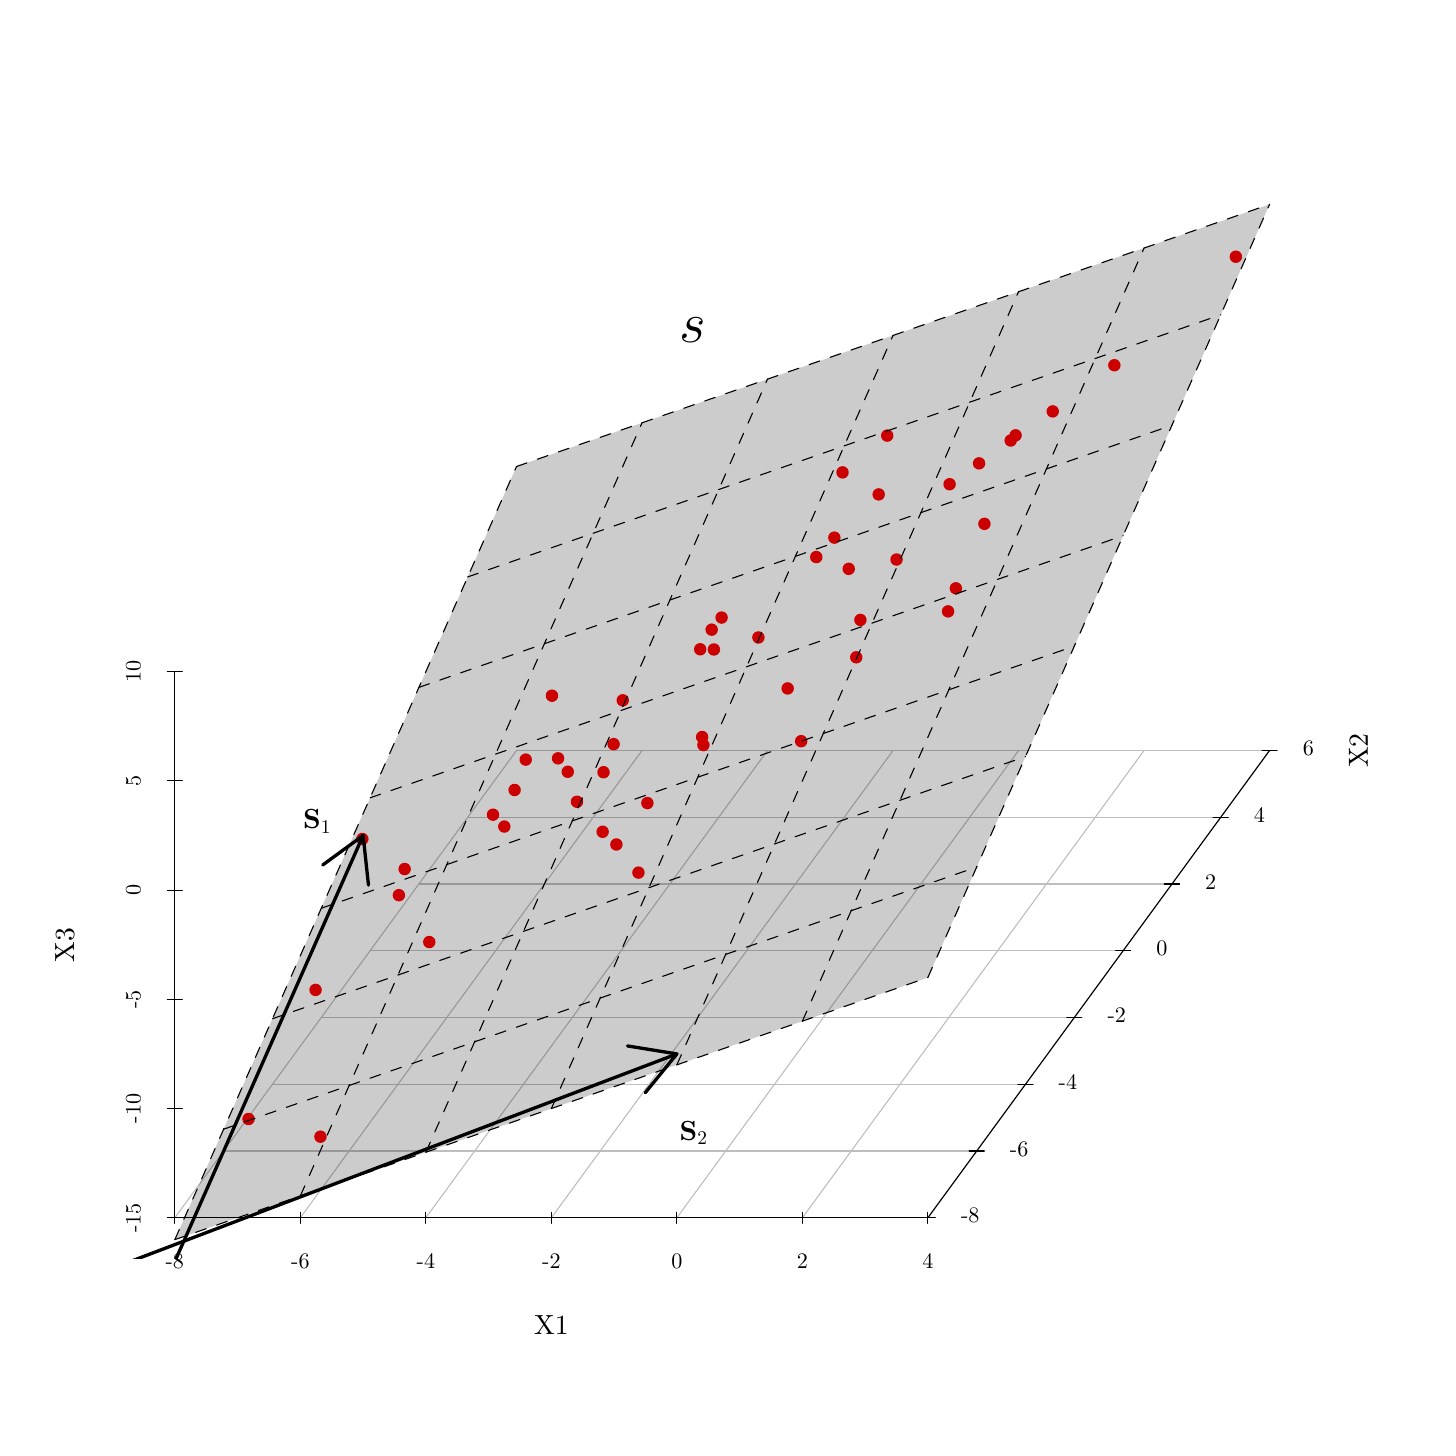
\begin{tikzpicture}[x=1pt,y=1pt]
\definecolor{fillColor}{RGB}{255,255,255}
\path[use as bounding box,fill=fillColor,fill opacity=0.00] (0,0) rectangle (505.89,505.89);
\begin{scope}
\path[clip] ( 37.20, 61.20) rectangle (468.69,456.69);
\definecolor{drawColor}{RGB}{190,190,190}

\path[draw=drawColor,line width= 0.4pt,line join=round,line cap=round] ( 53.18, 75.85) -- (176.64,244.69);

\path[draw=drawColor,line width= 0.4pt,line join=round,line cap=round] ( 98.53, 75.85) -- (221.99,244.69);

\path[draw=drawColor,line width= 0.4pt,line join=round,line cap=round] (143.88, 75.85) -- (267.34,244.69);

\path[draw=drawColor,line width= 0.4pt,line join=round,line cap=round] (189.24, 75.85) -- (312.69,244.69);

\path[draw=drawColor,line width= 0.4pt,line join=round,line cap=round] (234.59, 75.85) -- (358.05,244.69);

\path[draw=drawColor,line width= 0.4pt,line join=round,line cap=round] (279.94, 75.85) -- (403.40,244.69);

\path[draw=drawColor,line width= 0.4pt,line join=round,line cap=round] (325.29, 75.85) -- (448.75,244.69);

\path[draw=drawColor,line width= 0.4pt,line join=round,line cap=round] ( 53.18, 75.85) -- (325.29, 75.85);

\path[draw=drawColor,line width= 0.4pt,line join=round,line cap=round] ( 70.82, 99.97) -- (342.93, 99.97);

\path[draw=drawColor,line width= 0.4pt,line join=round,line cap=round] ( 88.45,124.09) -- (360.57,124.09);

\path[draw=drawColor,line width= 0.4pt,line join=round,line cap=round] (106.09,148.21) -- (378.20,148.21);

\path[draw=drawColor,line width= 0.4pt,line join=round,line cap=round] (123.73,172.33) -- (395.84,172.33);

\path[draw=drawColor,line width= 0.4pt,line join=round,line cap=round] (141.37,196.45) -- (413.48,196.45);

\path[draw=drawColor,line width= 0.4pt,line join=round,line cap=round] (159.00,220.57) -- (431.11,220.57);

\path[draw=drawColor,line width= 0.4pt,line join=round,line cap=round] (176.64,244.69) -- (448.75,244.69);
\definecolor{drawColor}{RGB}{0,0,0}

\path[draw=drawColor,line width= 0.4pt,line join=round,line cap=round] (322.57, 75.85) -- (328.01, 75.85);

\path[draw=drawColor,line width= 0.4pt,line join=round,line cap=round] (340.21, 99.97) -- (345.65, 99.97);

\path[draw=drawColor,line width= 0.4pt,line join=round,line cap=round] (357.84,124.09) -- (363.29,124.09);

\path[draw=drawColor,line width= 0.4pt,line join=round,line cap=round] (375.48,148.21) -- (380.92,148.21);

\path[draw=drawColor,line width= 0.4pt,line join=round,line cap=round] (393.12,172.33) -- (398.56,172.33);

\path[draw=drawColor,line width= 0.4pt,line join=round,line cap=round] (410.75,196.45) -- (416.20,196.45);

\path[draw=drawColor,line width= 0.4pt,line join=round,line cap=round] (428.39,220.57) -- (433.83,220.57);

\path[draw=drawColor,line width= 0.4pt,line join=round,line cap=round] (446.03,244.69) -- (451.47,244.69);

\path[draw=drawColor,line width= 0.4pt,line join=round,line cap=round] ( 53.18, 73.87) -- ( 53.18, 77.82);

\path[draw=drawColor,line width= 0.4pt,line join=round,line cap=round] ( 98.53, 73.87) -- ( 98.53, 77.82);

\path[draw=drawColor,line width= 0.4pt,line join=round,line cap=round] (143.88, 73.87) -- (143.88, 77.82);

\path[draw=drawColor,line width= 0.4pt,line join=round,line cap=round] (189.24, 73.87) -- (189.24, 77.82);

\path[draw=drawColor,line width= 0.4pt,line join=round,line cap=round] (234.59, 73.87) -- (234.59, 77.82);

\path[draw=drawColor,line width= 0.4pt,line join=round,line cap=round] (279.94, 73.87) -- (279.94, 77.82);

\path[draw=drawColor,line width= 0.4pt,line join=round,line cap=round] (325.29, 73.87) -- (325.29, 77.82);

\path[draw=drawColor,line width= 0.4pt,line join=round,line cap=round] ( 50.46, 75.85) -- ( 55.90, 75.85);

\path[draw=drawColor,line width= 0.4pt,line join=round,line cap=round] ( 50.46,115.32) -- ( 55.90,115.32);

\path[draw=drawColor,line width= 0.4pt,line join=round,line cap=round] ( 50.46,154.79) -- ( 55.90,154.79);

\path[draw=drawColor,line width= 0.4pt,line join=round,line cap=round] ( 50.46,194.26) -- ( 55.90,194.26);

\path[draw=drawColor,line width= 0.4pt,line join=round,line cap=round] ( 50.46,233.73) -- ( 55.90,233.73);

\path[draw=drawColor,line width= 0.4pt,line join=round,line cap=round] ( 50.46,273.20) -- ( 55.90,273.20);
\end{scope}
\begin{scope}
\path[clip] (  0.00,  0.00) rectangle (505.89,505.89);
\definecolor{drawColor}{RGB}{0,0,0}

\node[text=drawColor,anchor=base,inner sep=0pt, outer sep=0pt, scale=  0.80] at ( 53.18, 57.60) {-8};

\node[text=drawColor,anchor=base,inner sep=0pt, outer sep=0pt, scale=  0.80] at ( 98.53, 57.60) {-6};

\node[text=drawColor,anchor=base,inner sep=0pt, outer sep=0pt, scale=  0.80] at (143.88, 57.60) {-4};

\node[text=drawColor,anchor=base,inner sep=0pt, outer sep=0pt, scale=  0.80] at (189.24, 57.60) {-2};

\node[text=drawColor,anchor=base,inner sep=0pt, outer sep=0pt, scale=  0.80] at (234.59, 57.60) { 0};

\node[text=drawColor,anchor=base,inner sep=0pt, outer sep=0pt, scale=  0.80] at (279.94, 57.60) { 2};

\node[text=drawColor,anchor=base,inner sep=0pt, outer sep=0pt, scale=  0.80] at (325.29, 57.60) { 4};

\node[text=drawColor,rotate= 90.00,anchor=base,inner sep=0pt, outer sep=0pt, scale=  0.80] at ( 40.80, 75.85) {-15};

\node[text=drawColor,rotate= 90.00,anchor=base,inner sep=0pt, outer sep=0pt, scale=  0.80] at ( 40.80,115.32) {-10};

\node[text=drawColor,rotate= 90.00,anchor=base,inner sep=0pt, outer sep=0pt, scale=  0.80] at ( 40.80,154.79) { -5};

\node[text=drawColor,rotate= 90.00,anchor=base,inner sep=0pt, outer sep=0pt, scale=  0.80] at ( 40.80,194.26) {  0};

\node[text=drawColor,rotate= 90.00,anchor=base,inner sep=0pt, outer sep=0pt, scale=  0.80] at ( 40.80,233.73) {  5};

\node[text=drawColor,rotate= 90.00,anchor=base,inner sep=0pt, outer sep=0pt, scale=  0.80] at ( 40.80,273.20) { 10};
\end{scope}
\begin{scope}
\path[clip] ( 37.20, 61.20) rectangle (468.69,456.69);
\definecolor{drawColor}{RGB}{0,0,0}

\node[text=drawColor,anchor=base west,inner sep=0pt, outer sep=0pt, scale=  0.80] at (337.29, 74.01) {-8};

\node[text=drawColor,anchor=base west,inner sep=0pt, outer sep=0pt, scale=  0.80] at (354.93, 98.13) {-6};

\node[text=drawColor,anchor=base west,inner sep=0pt, outer sep=0pt, scale=  0.80] at (372.57,122.25) {-4};

\node[text=drawColor,anchor=base west,inner sep=0pt, outer sep=0pt, scale=  0.80] at (390.20,146.37) {-2};

\node[text=drawColor,anchor=base west,inner sep=0pt, outer sep=0pt, scale=  0.80] at (407.84,170.49) { 0};

\node[text=drawColor,anchor=base west,inner sep=0pt, outer sep=0pt, scale=  0.80] at (425.48,194.61) { 2};

\node[text=drawColor,anchor=base west,inner sep=0pt, outer sep=0pt, scale=  0.80] at (443.11,218.73) { 4};

\node[text=drawColor,anchor=base west,inner sep=0pt, outer sep=0pt, scale=  0.80] at (460.75,242.86) { 6};

\path[draw=drawColor,line width= 0.4pt,line join=round,line cap=round] ( 53.18, 75.85) --
	(325.29, 75.85);
\end{scope}
\begin{scope}
\path[clip] (  0.00,  0.00) rectangle (505.89,505.89);
\definecolor{drawColor}{RGB}{0,0,0}

\node[text=drawColor,anchor=base,inner sep=0pt, outer sep=0pt, scale=  1.00] at (189.24, 33.60) {X1};
\end{scope}
\begin{scope}
\path[clip] ( 37.20, 61.20) rectangle (468.69,456.69);
\definecolor{drawColor}{RGB}{0,0,0}

\path[draw=drawColor,line width= 0.4pt,line join=round,line cap=round] (325.29, 75.85) --
	(448.75,244.69);
\end{scope}
\begin{scope}
\path[clip] (  0.00,  0.00) rectangle (505.89,505.89);
\definecolor{drawColor}{RGB}{0,0,0}

\node[text=drawColor,rotate= 90.00,anchor=base,inner sep=0pt, outer sep=0pt, scale=  1.00] at (484.29,244.69) {X2};
\end{scope}
\begin{scope}
\path[clip] ( 37.20, 61.20) rectangle (468.69,456.69);
\definecolor{drawColor}{RGB}{0,0,0}

\path[draw=drawColor,line width= 0.4pt,line join=round,line cap=round] ( 53.18, 75.85) --
	( 53.18,273.20);
\end{scope}
\begin{scope}
\path[clip] (  0.00,  0.00) rectangle (505.89,505.89);
\definecolor{drawColor}{RGB}{0,0,0}

\node[text=drawColor,rotate= 90.00,anchor=base,inner sep=0pt, outer sep=0pt, scale=  1.00] at ( 16.80,174.52) {X3};
\end{scope}
\begin{scope}
\path[clip] ( 37.20, 61.20) rectangle (468.69,456.69);
\definecolor{fillColor}{RGB}{255,0,0}

\path[fill=fillColor] (436.57,423.12) circle (  2.25);

\path[fill=fillColor] (310.59,358.48) circle (  2.25);

\path[fill=fillColor] (392.67,383.91) circle (  2.25);

\path[fill=fillColor] (294.45,345.19) circle (  2.25);

\path[fill=fillColor] (370.39,367.23) circle (  2.25);

\path[fill=fillColor] (356.98,358.58) circle (  2.25);

\path[fill=fillColor] (355.21,356.71) circle (  2.25);

\path[fill=fillColor] (307.51,337.23) circle (  2.25);

\path[fill=fillColor] (343.78,348.45) circle (  2.25);

\path[fill=fillColor] (333.13,340.91) circle (  2.25);

\path[fill=fillColor] (291.49,321.61) circle (  2.25);

\path[fill=fillColor] (284.96,314.59) circle (  2.25);

\path[fill=fillColor] (296.68,310.34) circle (  2.25);

\path[fill=fillColor] (345.72,326.59) circle (  2.25);

\path[fill=fillColor] (250.75,292.73) circle (  2.25);

\path[fill=fillColor] (313.96,313.70) circle (  2.25);

\path[fill=fillColor] (247.16,288.36) circle (  2.25);

\path[fill=fillColor] (189.45,264.50) circle (  2.25);

\path[fill=fillColor] (243.02,281.27) circle (  2.25);

\path[fill=fillColor] (247.96,281.19) circle (  2.25);

\path[fill=fillColor] (264.05,285.54) circle (  2.25);

\path[fill=fillColor] (215.03,262.83) circle (  2.25);

\path[fill=fillColor] (300.90,291.88) circle (  2.25);

\path[fill=fillColor] (335.40,303.30) circle (  2.25);

\path[fill=fillColor] (332.58,294.96) circle (  2.25);

\path[fill=fillColor] (179.97,241.40) circle (  2.25);

\path[fill=fillColor] (191.66,241.87) circle (  2.25);

\path[fill=fillColor] (299.40,278.37) circle (  2.25);

\path[fill=fillColor] (211.73,246.99) circle (  2.25);

\path[fill=fillColor] (274.62,267.12) circle (  2.25);

\path[fill=fillColor] (120.93,212.71) circle (  2.25);

\path[fill=fillColor] (175.95,230.42) circle (  2.25);

\path[fill=fillColor] (195.16,237.01) circle (  2.25);

\path[fill=fillColor] (243.71,249.56) circle (  2.25);

\path[fill=fillColor] (208.09,236.84) circle (  2.25);

\path[fill=fillColor] (168.15,221.49) circle (  2.25);

\path[fill=fillColor] (244.17,246.66) circle (  2.25);

\path[fill=fillColor] (172.23,217.21) circle (  2.25);

\path[fill=fillColor] (198.50,226.18) circle (  2.25);

\path[fill=fillColor] (136.21,201.87) circle (  2.25);

\path[fill=fillColor] (279.49,248.06) circle (  2.25);

\path[fill=fillColor] (223.93,225.70) circle (  2.25);

\path[fill=fillColor] (134.14,192.41) circle (  2.25);

\path[fill=fillColor] (207.76,215.33) circle (  2.25);

\path[fill=fillColor] (212.73,210.74) circle (  2.25);

\path[fill=fillColor] (145.12,175.48) circle (  2.25);

\path[fill=fillColor] (220.70,200.57) circle (  2.25);

\path[fill=fillColor] (104.03,158.19) circle (  2.25);

\path[fill=fillColor] ( 79.81,111.54) circle (  2.25);

\path[fill=fillColor] (105.79,105.14) circle (  2.25);
\definecolor{fillColor}{RGB}{0,0,0}

\path[fill=fillColor,fill opacity=0.20] ( 53.18, 67.95) --
	(176.64,347.31) --
	(448.75,442.04) --
	(325.29,162.68) --
	cycle;
\definecolor{drawColor}{RGB}{0,0,0}

\path[draw=drawColor,line width= 0.4pt,dash pattern=on 4pt off 4pt ,line join=round,line cap=round] ( 53.18, 67.95) -- (176.64,347.31);

\path[draw=drawColor,line width= 0.4pt,dash pattern=on 4pt off 4pt ,line join=round,line cap=round] ( 98.53, 83.74) -- (221.99,363.10);

\path[draw=drawColor,line width= 0.4pt,dash pattern=on 4pt off 4pt ,line join=round,line cap=round] (143.88, 99.53) -- (267.34,378.89);

\path[draw=drawColor,line width= 0.4pt,dash pattern=on 4pt off 4pt ,line join=round,line cap=round] (189.24,115.32) -- (312.69,394.68);

\path[draw=drawColor,line width= 0.4pt,dash pattern=on 4pt off 4pt ,line join=round,line cap=round] (234.59,131.11) -- (358.05,410.47);

\path[draw=drawColor,line width= 0.4pt,dash pattern=on 4pt off 4pt ,line join=round,line cap=round] (279.94,146.89) -- (403.40,426.25);

\path[draw=drawColor,line width= 0.4pt,dash pattern=on 4pt off 4pt ,line join=round,line cap=round] (325.29,162.68) -- (448.75,442.04);

\path[draw=drawColor,line width= 0.4pt,dash pattern=on 4pt off 4pt ,line join=round,line cap=round] ( 53.18, 67.95) -- (325.29,162.68);

\path[draw=drawColor,line width= 0.4pt,dash pattern=on 4pt off 4pt ,line join=round,line cap=round] ( 70.82,107.86) -- (342.93,202.59);

\path[draw=drawColor,line width= 0.4pt,dash pattern=on 4pt off 4pt ,line join=round,line cap=round] ( 88.45,147.77) -- (360.57,242.50);

\path[draw=drawColor,line width= 0.4pt,dash pattern=on 4pt off 4pt ,line join=round,line cap=round] (106.09,187.68) -- (378.20,282.41);

\path[draw=drawColor,line width= 0.4pt,dash pattern=on 4pt off 4pt ,line join=round,line cap=round] (123.73,227.59) -- (395.84,322.32);

\path[draw=drawColor,line width= 0.4pt,dash pattern=on 4pt off 4pt ,line join=round,line cap=round] (141.37,267.50) -- (413.48,362.22);

\path[draw=drawColor,line width= 0.4pt,dash pattern=on 4pt off 4pt ,line join=round,line cap=round] (159.00,307.41) -- (431.11,402.13);

\path[draw=drawColor,line width= 0.4pt,dash pattern=on 4pt off 4pt ,line join=round,line cap=round] (176.64,347.31) -- (448.75,442.04);

\path[draw=drawColor,line width= 1.2pt,line join=round,line cap=round] ( 26.64,  0.00) -- (121.21,213.99);

\path[draw=drawColor,line width= 1.2pt,line join=round,line cap=round] (123.15,196.03) --
	(121.21,213.99) --
	(106.62,203.33);

\path[draw=drawColor,line width= 1.2pt,line join=round,line cap=round] (  0.00, 45.96) -- (234.59,135.05);

\path[draw=drawColor,line width= 1.2pt,line join=round,line cap=round] (223.17,121.05) --
	(234.59,135.05) --
	(216.75,137.94);

\node[text=drawColor,anchor=base west,inner sep=0pt, outer sep=0pt, scale=  1.00] at ( 99.52,216.34) {\bfseries S};

\node[text=drawColor,anchor=base west,inner sep=0pt, outer sep=0pt, scale=  0.70] at (105.91,214.83) {1};

\node[text=drawColor,anchor=base west,inner sep=0pt, outer sep=0pt, scale=  1.00] at (235.58,103.85) {\bfseries S};

\node[text=drawColor,anchor=base west,inner sep=0pt, outer sep=0pt, scale=  0.70] at (241.96,102.34) {2};

\node[text=drawColor,anchor=base west,inner sep=0pt, outer sep=0pt, scale=  1.00] at (235.51,392.30) {{\huge $\mathfrak{s}$}};
\end{scope}
\end{tikzpicture}
